\documentclass[12pt]{article}
\usepackage[utf8]{inputenc}
%\usepackage[portuguese]{babel}
\usepackage{amsmath,amsfonts,amssymb}
\usepackage{graphicx}
\usepackage{makeidx}
\usepackage{graphicx}
\usepackage{lmodern}
\usepackage{multicol}
\usepackage{booktabs}
\usepackage{fancyhdr}
\usepackage{hyperref}
\usepackage[usenames]{color}


\usepackage{Sweave}
\begin{document}
\Sconcordance{concordance:knn.tex:knn.Rnw:%
1 15 1 1 0 43 1 1 2 1 0 1 5 4 0 1 25 26 0 1 2 8 1 1 19 18 0 2 1 1 2 1 0 %
1 1 3 0 1 2 1 1 1 14 16 0 1 2 3 1 1 8 10 0 1 2 2 1 1 3 1 2 3 1 1 4 2 1 %
1 3 1 2 5 1 1 3 1 2 5 1 1 3 1 2 6 1 1 8 2 1 1 3 1 2 3 1 1 4 2 1 1 3 1 2 %
5 1 1 3 1 2 5 1 1 3 1 2 4 1 1 8 2 1 1 3 1 2 3 1 1 4 2 1 1 3 1 2 5 1 1 3 %
1 2 5 1 1 3 1 2 23 1}

\pagestyle{fancy}
\fancyhf{}
\renewcommand{\headrulewidth}{0.4pt}
\fancyfoot[C]{\thepage}
\renewcommand{\footrulewidth}{0.4pt}
\fancyfoot[C]{\thepage}
\title{\LARGE \bf
 Exercício 3 -  K-Nearest Neighbors}
\author{ Rodrigo Machado Fonseca - 2017002253}
\thispagestyle{fancy}
\fancyhead[C]{Introdução ao Reconhecimento de Padrões - UFMG \\ Belo Horizonte - \today}
\maketitle
\thispagestyle{fancy}

%%%%%%%%%%%%%%%%%%%%%%%%%%%%%%%%%%%%%%%%%%%%%%%%%%%%%%%%%%%%%%%%%%%%%%%%%%%%%%%%%%%%%%%%%
\section{Introdução}

  \par Neste trabalho iremos implementar o algoritmo \textit{k-Nearest Neighbors} na seção \ref{knn}. Em seguida, iremos utilizá-lo para classificar um conjunto de amostras. 
  
\section{K-Nearest Neighbors}
  \label{knn}
  \par O algoritmo \textit{k-Nearest Neighbors} é um classificador que utiliza métricas de distâncias para classificar novas amostras. Para entendermos como funcionar vamos analisar o conjunto de passos:

  \begin{itemize}
    \item Recebe uma amostra e calcula a distância para todas as amostras que já estão rotuladas. 
    \item Ordena em ordem crescente de acordo com a distância calculada.
    \item Escolhe as k primeiras amostras.
    \item Conta o número de rótulos dentro do grupo escolhido.
    \item Ordena em ordem decrescente. 
    \item Atribui como rótulo da nova amostra o primeiro rótulo da lista. 
  \end{itemize}

  \par Para aplicar o método basta termos um conjunto de amostras que já estão rotuladas e a partir do momento que recebemos um novo número de amostras, podemos implementar a sequência de passos acima que teremos uma classificação para nova amostras. 
  
  \par Para o cálculo da distância utilizaremos a fórmula da distância Euclidiana. 
  
  \par Pode acontecer um empate de rótulos dentro do conjunto k escolhido. Para isso adotamos a solução utilizada pelo algoritmo \ref{matlab}, que dentre os rótulos mais frequentes, escolhe um de forma aleatória. 

\section{Implementação KNN}

  \par Agora que já explicamos  conceitualmente os passos do algoritmo KNN iremos implementar o passo a passo descrito na seção \ref{knn}.
  
\begin{Schunk}
\begin{Sinput}
> rm(list=ls())
> calculate_distance <- function(line_matrix, mn_matrix, p){
+   line_matrix <- as.matrix(line_matrix, nrow=1)
+   difference <- t(apply(mn_matrix[,1:2], 1,'-', line_matrix))
+   return(rowSums(abs(difference)^p)^(1/p))
+ }
> knn <- function(comparison_matrix, sample_matrix, k, p){
+     labels_clusters <- comparison_matrix[,3]
+     base_matrix <-  comparison_matrix[,1:2]
+     labels_output <- matrix(nrow = dim(sample_matrix)[1], ncol = 1)
+     sample_matrix <- sample_matrix[,1:2]
+     for(i in 1:dim(sample_matrix)[1]){
+       distance <- calculate_distance(sample_matrix[i,],
+                                      comparison_matrix, p)
+       indexes <- sort(distance,
+                       index.return=TRUE)[[2]][1:k]
+       select_label <- labels_clusters[indexes]
+       table_label <- table(select_label)
+       if(length(strtoi(names(
+         table_label[table_label == max(table_label)])))> 1){
+          labels_output[i,1] <- sample(strtoi(names(
+            table_label[table_label == max(table_label)])), 1)
+       }else{
+         labels_output[i,1] <- strtoi(
+           names(table_label[table_label == max(table_label)]))
+       }
+       
+     }
+     return(cbind(sample_matrix, labels_output))
+ }
\end{Sinput}
\end{Schunk}

\section{Metodologia}
  \par Para fazermos o treinamento iremos  criar 4 gaussianas com o mesmo desvio padrão, com 100 pontos cada e com os centros nos pontos (2,2), (2,4), (4,2), (4,4). Essas receberam rótulos de 1 a 4. 
  
  \par Além disso, criaremos um conjunto aleatório de 20 amostras com distribuição uniforme, as quais iremos classificar. Será atribuído um rótulo igual a 6 apenas para as amostras ficarem coerente com a função \textit{plot\_samples}.

  \par Os procedimentos citados no parágrafo anterior serão repetidos três vezes um para cada respectivo valor de desvio padrão: 0.3; 0.5; 0.7.
  
  \par Para cada conjunto gaussianas e amostras iremos classificar utilizando os valores de k igual a 2, 4 e 8. 
\begin{Schunk}
\begin{Sinput}
> build_gaussians <- function(standard_deviation, sample_number){
+   s_d<-standard_deviation
+   nc<-sample_number
+   xc1 <- matrix(rnorm(nc*2), ncol=2)*s_d + t(matrix(c(2 ,2), nrow=2,ncol=nc))
+   xc2 <- matrix(rnorm(nc*2), ncol=2)*s_d + t(matrix(c(4 ,4), nrow=2,ncol=nc))
+   xc3 <- matrix(rnorm(nc*2), ncol=2)*s_d + t(matrix(c(2 ,4), nrow=2,ncol=nc))
+   xc4 <- matrix(rnorm(nc*2), ncol=2)*s_d + t(matrix(c(4 ,2), nrow=2,ncol=nc))
+   y1 <- array(1, c(nc,1))
+   y2 <- array(2, c(nc,1))
+   y3 <- array(3, c(nc,1))
+   y4 <- array(4, c(nc,1))
+   sample1 <- cbind(xc1, y1)
+   sample2 <- cbind(xc2, y2)
+   sample3 <- cbind(xc3, y3)
+   sample4 <- cbind(xc4, y4)
+   samples <- rbind(sample1, sample2, sample3, sample4)
+   return(samples)
+ }
> comparison_matrix <- build_gaussians(0.3, 100)
> nc <- 20
> sample_matrix <- matrix(runif(nc*2)-0.5, ncol=2) * 2 + t(matrix(c(3 ,3),
+                                                         nrow=2,ncol=nc))
> sample_matrix <- cbind(sample_matrix, matrix(data = 6, nrow = nc, ncol = 1))
\end{Sinput}
\end{Schunk}
  \par Para avaliarmos os resultados construimos uma função para plotar o conjunto de gaussianas juntamente com as amostras, e a utilizaremos, antes e após o treinamento. 
  
\begin{Schunk}
\begin{Sinput}
> plotter_samples <- function(comparison_matrix, sample_matrix){
+   plot(comparison_matrix[1:100, 1], comparison_matrix[1:100, 2],
+        col = comparison_matrix[1:100, 3], xlim = c(0,6), ylim = c(0,6),
+        xlab = "x1", ylab = "x2")
+   points (comparison_matrix[101:200, 1],
+           comparison_matrix[101:200, 2], col =comparison_matrix[101:200, 3])
+   points (comparison_matrix[201:300, 1],
+           comparison_matrix[201:300, 2], col =  comparison_matrix[201:300, 3])
+   points (comparison_matrix[301:400, 1],
+           comparison_matrix[301:400, 2], col =comparison_matrix[301:400, 3])
+   points (sample_matrix[,1],
+           sample_matrix[,2], col = sample_matrix[,3])
+ }
\end{Sinput}
\end{Schunk}

\section{Resultados}
  \par A seguir estão as figuras antes e após a classificação do algoritmo knn.
  
\begin{Schunk}
\begin{Sinput}
> calc_knns <- function(k, p, comparison_matrix, sample_matrix) {
+   knn_list <- list()
+   for(i in k){
+    knn_list <- c(knn_list, list(knn(comparison_matrix, sample_matrix, i, 2)))
+   }
+   return(knn_list)
+ }
\end{Sinput}
\end{Schunk}

\begin{figure}[h]
\centering
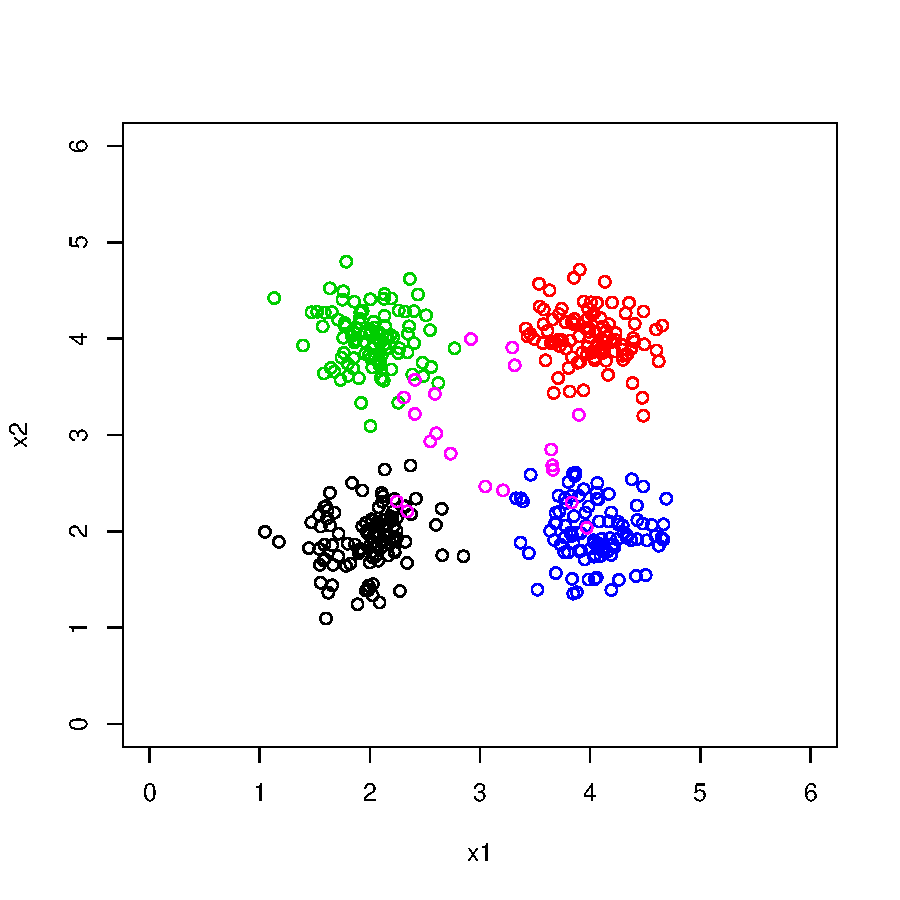
\includegraphics{knn-005}
\caption{Amostras antes da classificação KNN com distribuições gaussianas com desvio padrão 0.3}
\label{sd_0.3}
\end{figure}


\begin{figure}[h]
\centering
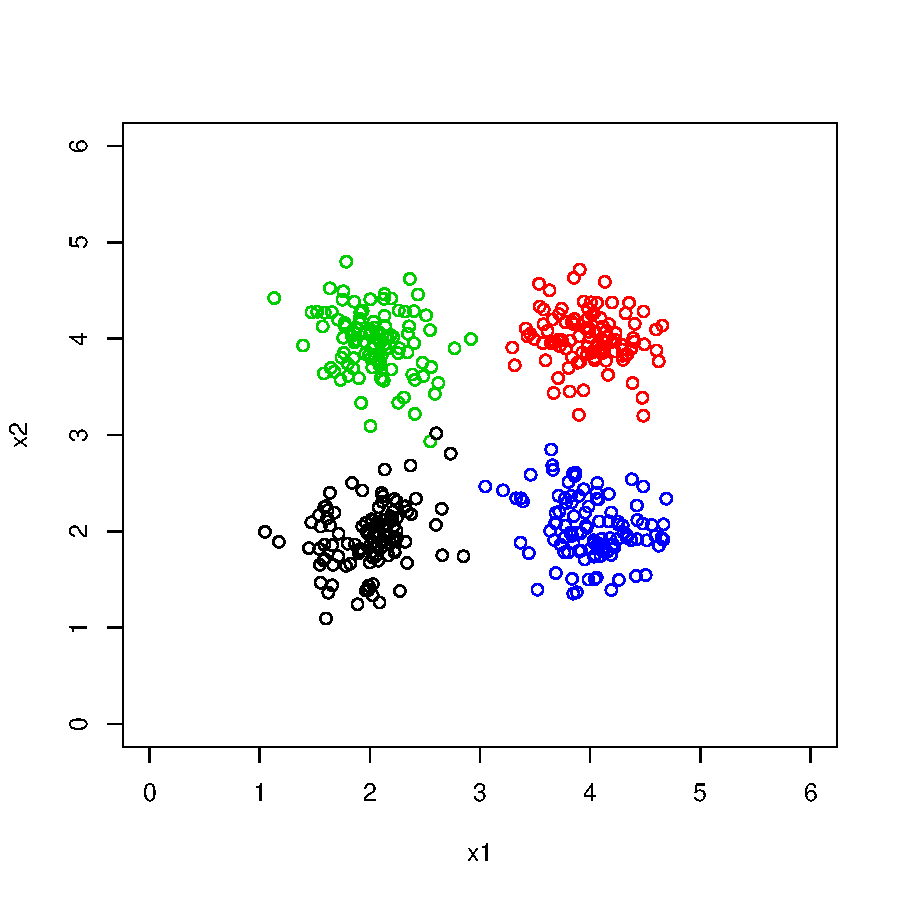
\includegraphics{knn-007}
\caption{Amostras após da classificação KNN com distribuições gaussianas com desvio padrão 0.3 e k igual a 2.}
\label{sd_0.3}
\end{figure}

\begin{figure}[h]
\centering
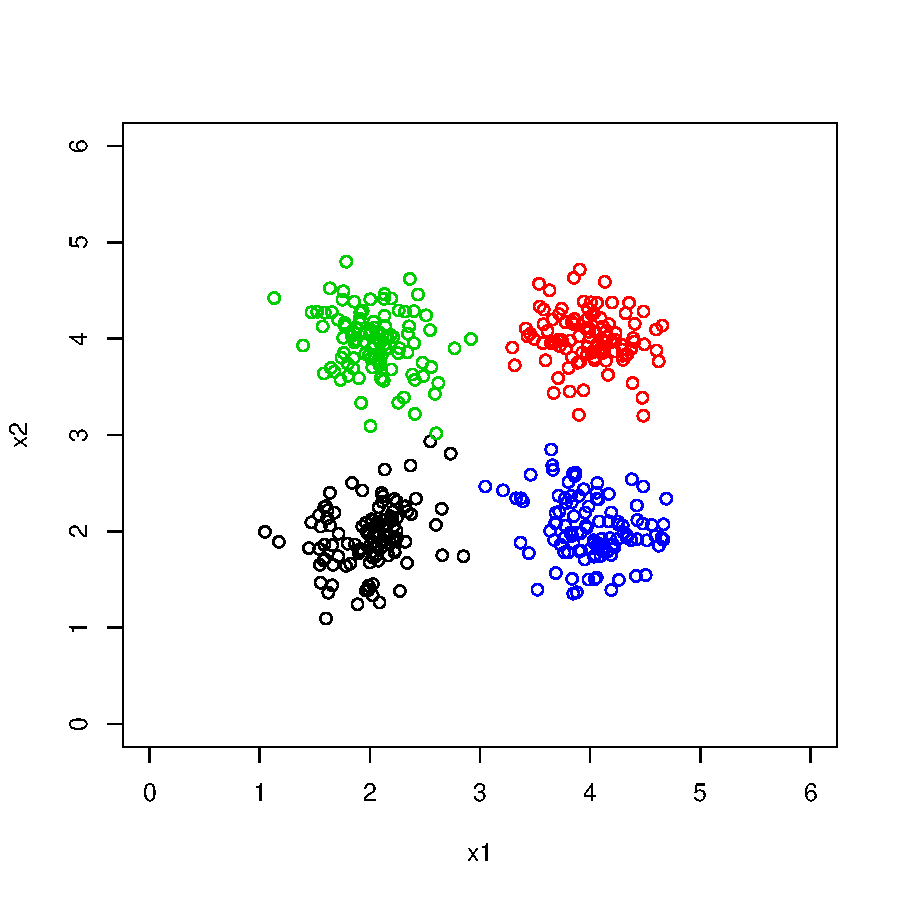
\includegraphics{knn-008}
\caption{Amostras após da classificação KNN com distribuições gaussianas com desvio padrão 0.3 e k igual a 4.}
\label{sd_0.3}
\end{figure}

\begin{figure}[h]
\centering
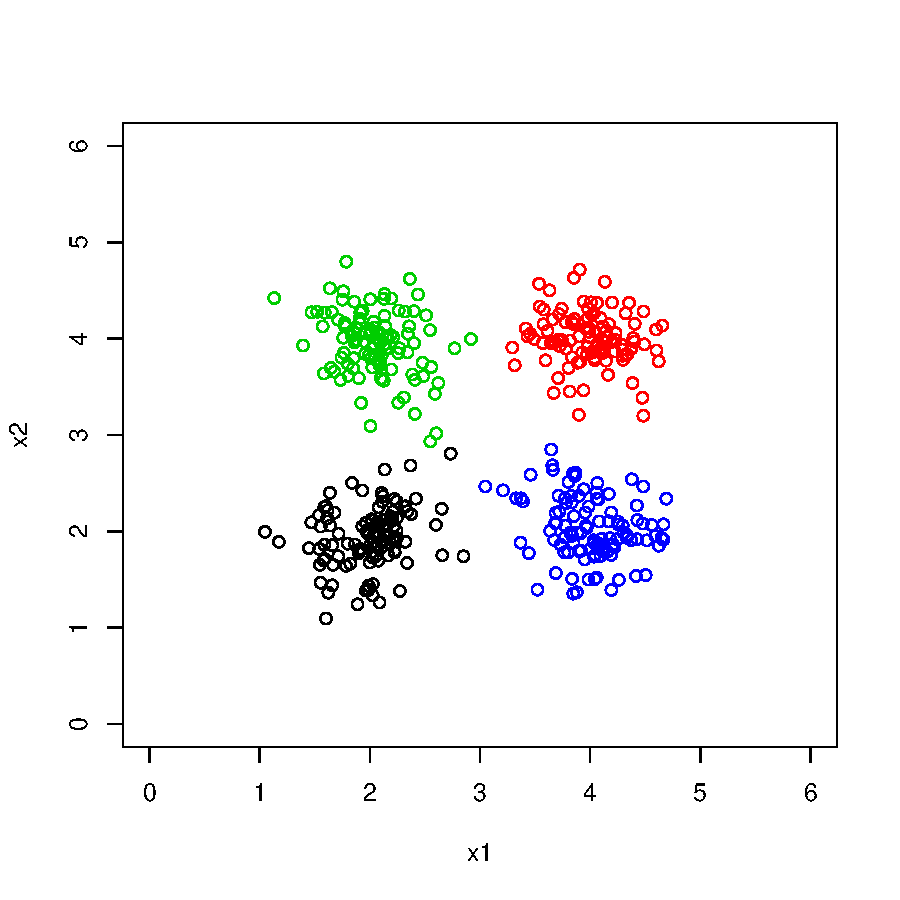
\includegraphics{knn-009}
\caption{Amostras após da classificação KNN com distribuições gaussianas com desvio padrão 0.3 e k igual a 8.}
\label{sd_0.3}
\end{figure}



%% Segunda parte 

\begin{figure}[h]
\centering
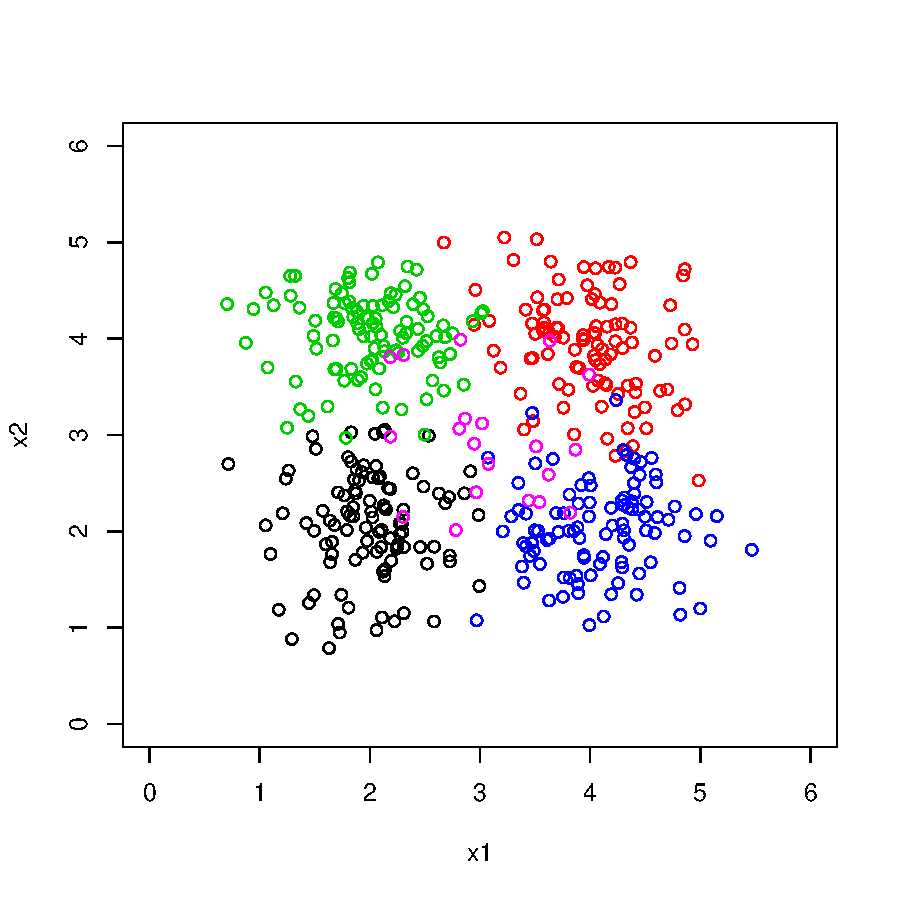
\includegraphics{knn-011}
\caption{Amostras antes da classificação KNN com distribuições gaussianas com desvio padrão 0.5}
\label{sd_0.5}
\end{figure}


\begin{figure}[h]
\centering
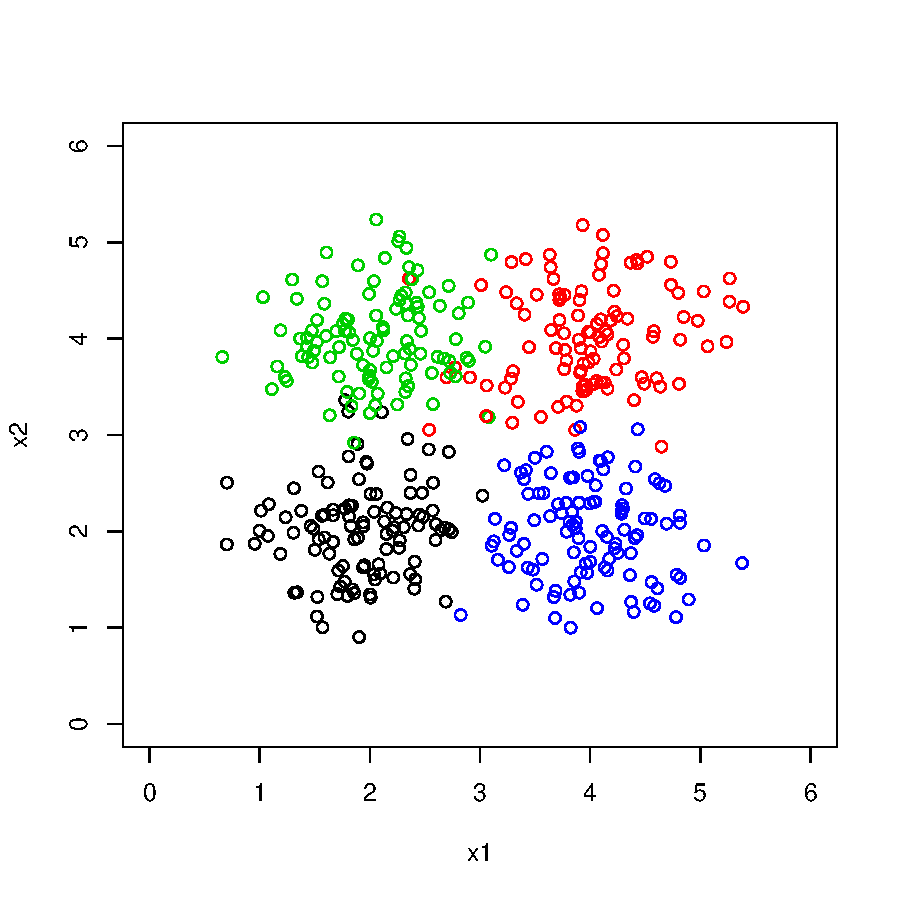
\includegraphics{knn-013}
\caption{Amostras após da classificação KNN com distribuições gaussianas com desvio padrão 0.5 e k igual a 2.}
\label{sd_0.5}
\end{figure}

\begin{figure}[h]
\centering
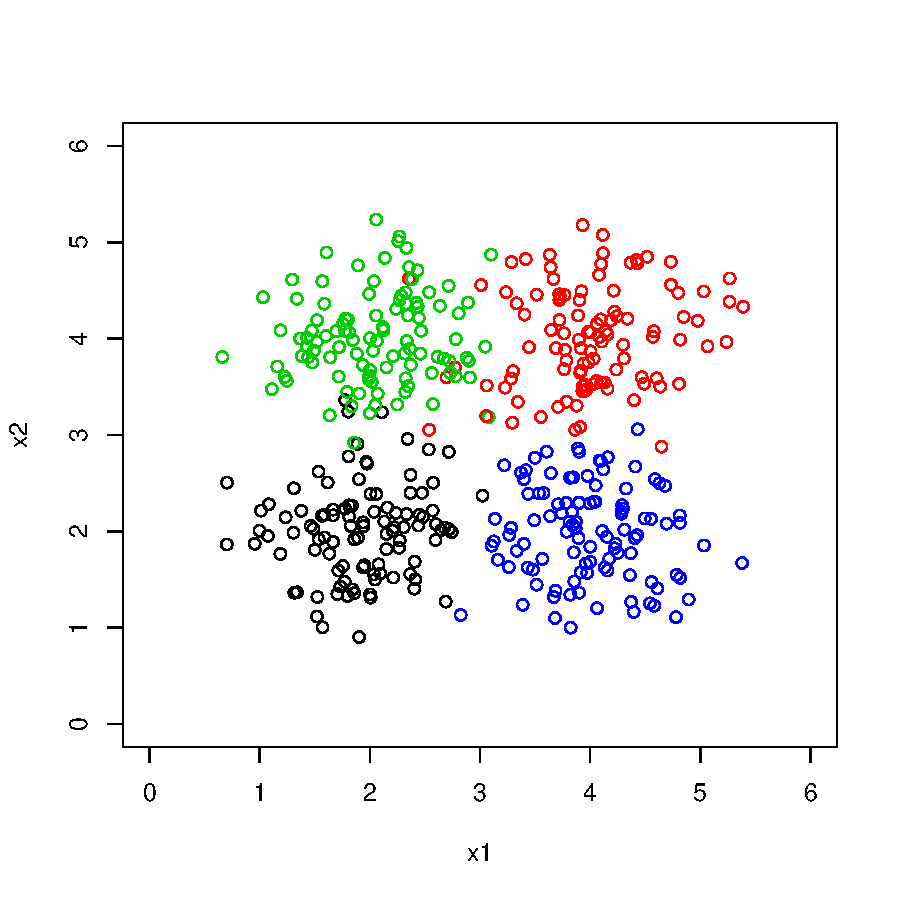
\includegraphics{knn-014}
\caption{Amostras após da classificação KNN com distribuições gaussianas com desvio padrão 0.5 e k igual a 4.}
\label{sd_0.5}
\end{figure}

\begin{figure}[h]
\centering
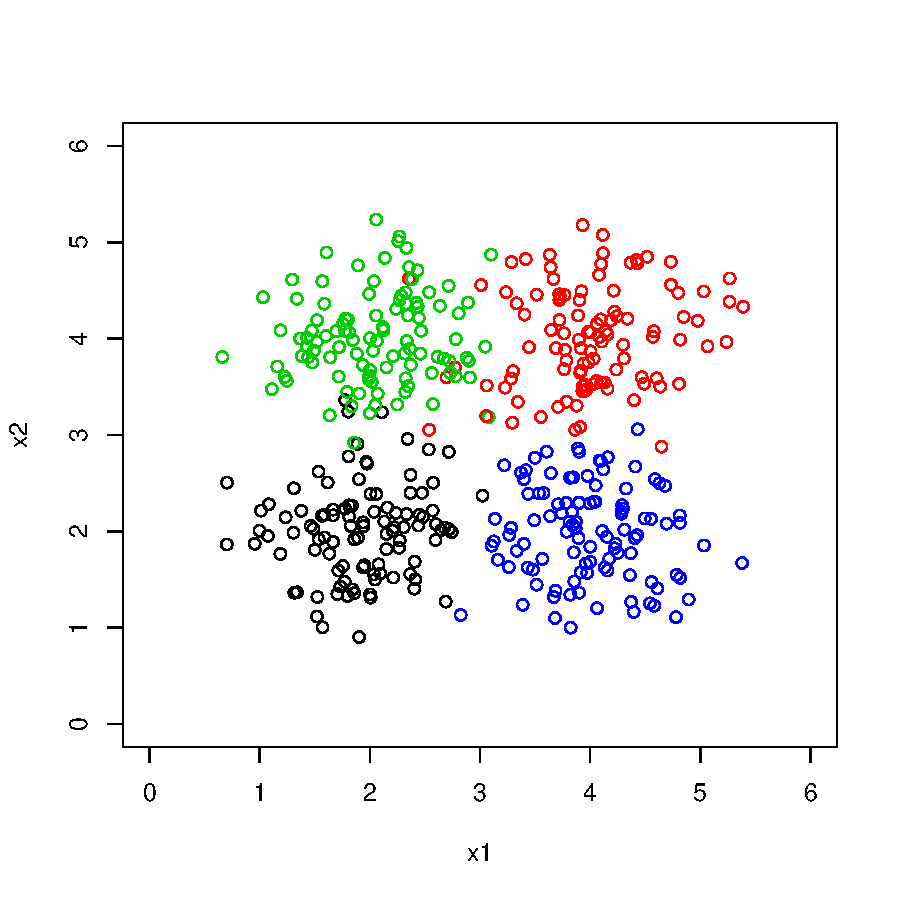
\includegraphics{knn-015}
\caption{Amostras após da classificação KNN com distribuições gaussianas com desvio padrão 0.5 e k igual a 8.}
\label{sd_0.5}
\end{figure}

%% Segunda parte 

\begin{figure}[h]
\centering
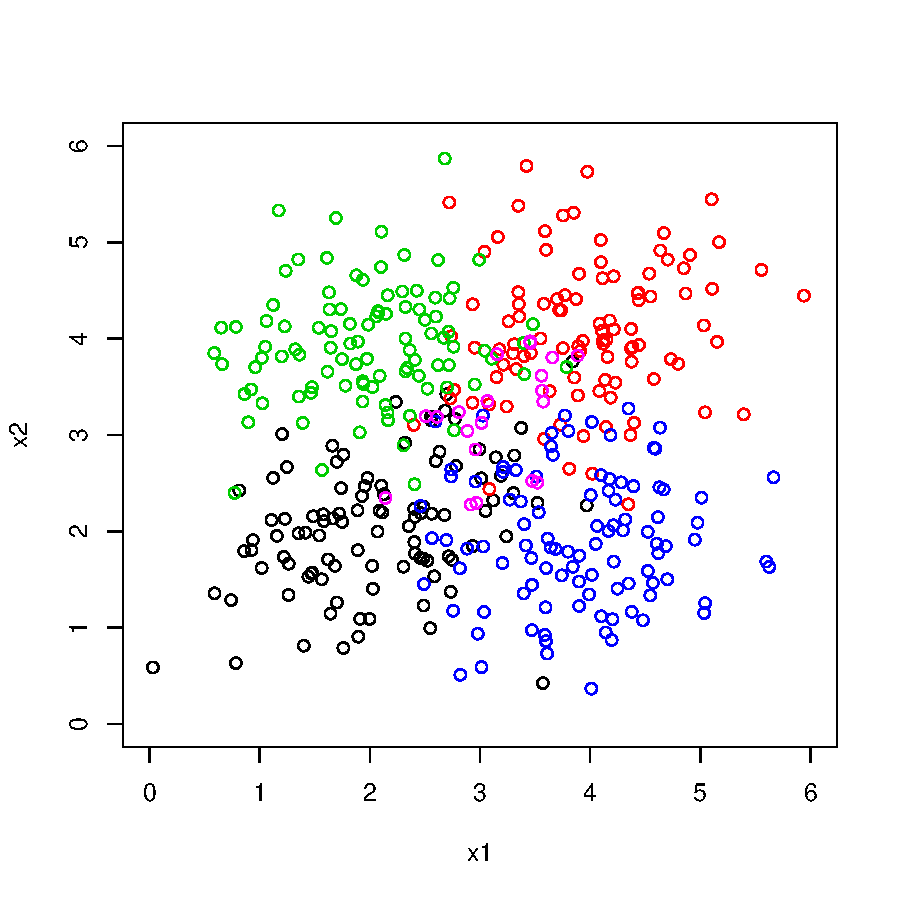
\includegraphics{knn-017}
\caption{Amostras antes da classificação KNN com distribuições gaussianas com desvio padrão 0.7}
\label{sd_0.7}
\end{figure}


\begin{figure}[h]
\centering
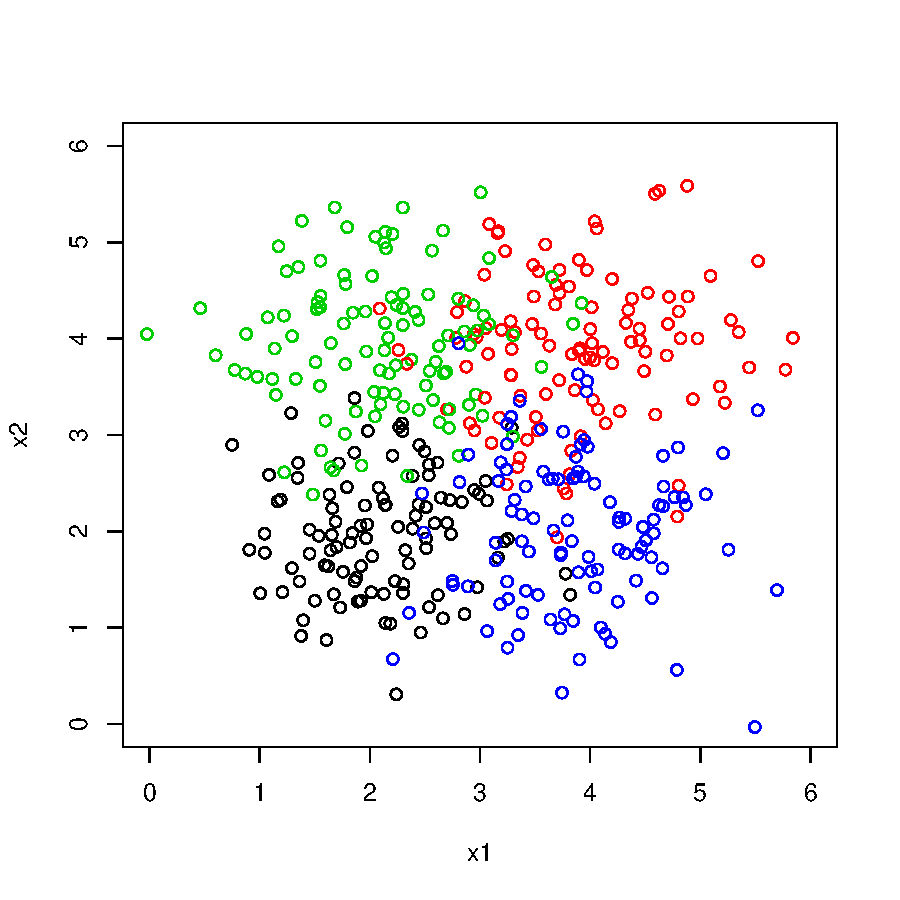
\includegraphics{knn-019}
\caption{Amostras após da classificação KNN com distribuições gaussianas com desvio padrão 0.7 e k igual a 2.}
\label{sd_0.7}
\end{figure}

\begin{figure}[h]
\centering
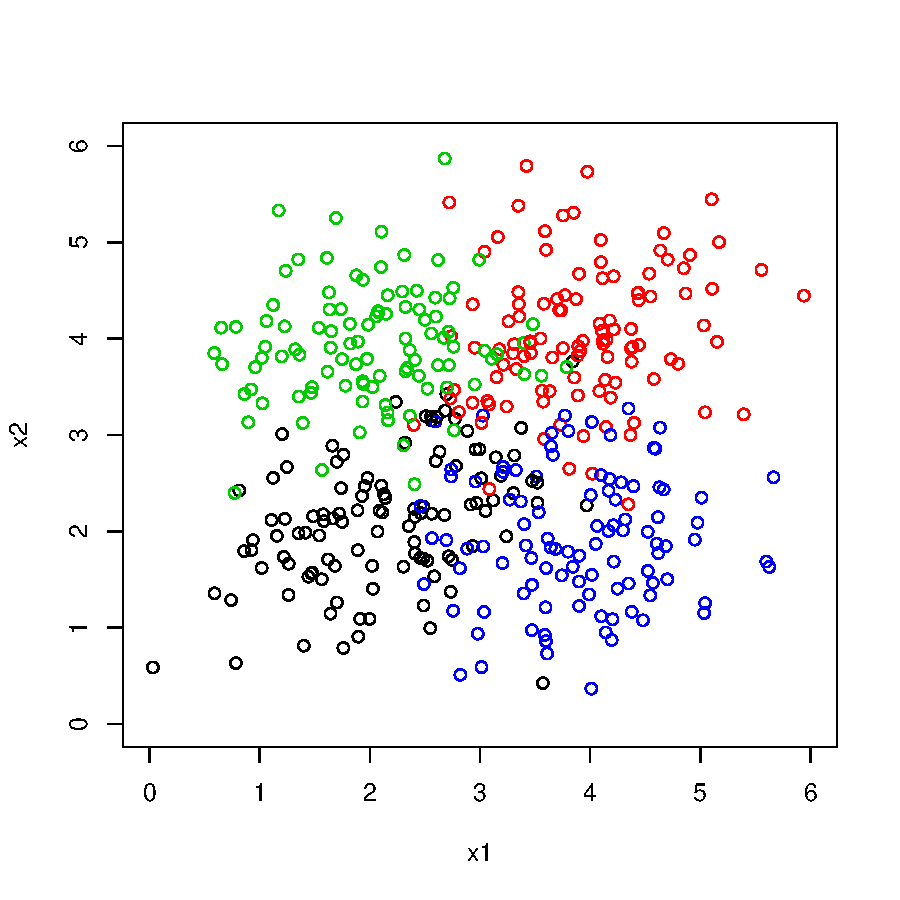
\includegraphics{knn-020}
\caption{Amostras após da classificação KNN com distribuições gaussianas com desvio padrão 0.7 e k igual a 4.}
\label{sd_0.7}
\end{figure}

\begin{figure}[h]
\centering
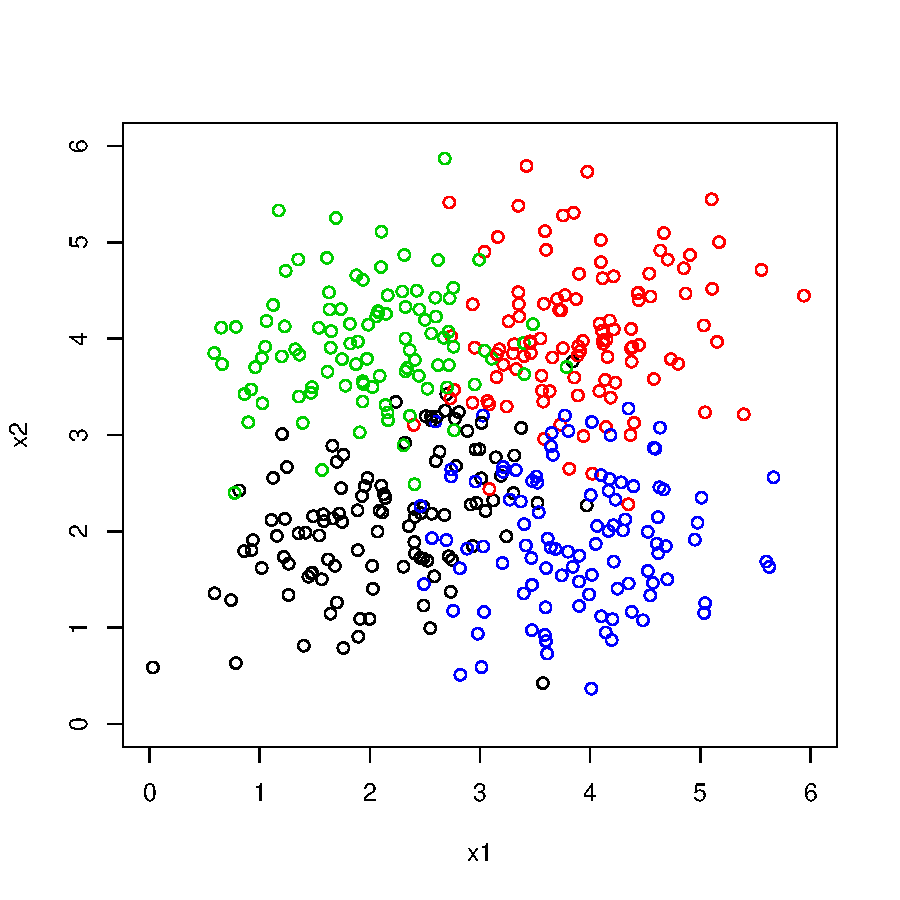
\includegraphics{knn-021}
\caption{Amostras após da classificação KNN com distribuições gaussianas com desvio padrão 0.7 e k igual a 8.}
\label{sd_0.7}
\end{figure}

\section{Discussão}
  \par Para o desvio padrão igual a 0.3 podemos observar que a separação é feita de maneira muito satisfatória e conseguimos agrupar de forma coerente as amostras. Além disso, podemos dividir o plano em 4 partes onde as retas seriam uma reta passa por x1=3 e paralela a x2, e uma reta passando por x2=3 e paralela a x1. Dessa forma, a melhor  forma de classificar as amostras mais próximas do centro seria sabendo a qual respectivo quadrante ela pertence. Analisando esse aspecto, podemos ver que ao aumentarmos k, as amostras são melhores classificadas de acordo com a gaussiana pertencente ao respectivo quadrante. 
  
  \par Para os valores de desvio padrão 0.5, torna-se um pouco mais complexo fazer a divisão, uma vez que há sobreposição de amostras de diferentes gaussianas. No entanto, podemos ver que a classificação é feita de forma satisfatória, principalmente com o aumento do valor de k. 
  
  \par Para os valores de desvio padrão 0.7, podemos ver que a classificação é a mais complexa e depende muito do local onde a amostra que será classificada está localizada, pois pode ser que a amostras caíam perto de um conjunto de amostras de um rótulo que estão mais dispersas das suas respectivas centróides. Neste caso, aumentar o valor de k não é muito eficiente, principalmente na região central (perto do ponto (3,3)).
  
  \par Ao final do experimento, pode-se afirmar que o objetivo do exercício foi cumprido, uma vez que foi possível implementar um algoritmo knn que é capaz de classificar um certo conjunto de amostras em um espaço formado por quatro classes. As figuras dos resultados nos permitem validar visualmente que o algoritmo está classificando corretamente as amostras. Além disso, foi possível observar também como os desvios-padrão das amostras de treinamento e o número de vizinhos mais próximos considerados na classificação alteram o resultado final do problema.
  \par Por fim, é relevante comentar que há outras formas de classificar as amostras que terminam empatadas. Uma possível solução seria variar o valor de p da distância de minkowski até a amostra convergir para um valor. Outrossim, utilizar valores k's iguais a impar iriam reduzir a probabilidade de empate. 
%%%%%%%%%%%%%%%%%%%%%%%%%%%%%%%%%%%%%%%%%%%%%%%%%%%%%%%%%%%%%%%%%%%%%%%%%%%%%%%%%%%%%%%%%

%%%%%%%%%%%%%%%%%%%%%%%%%%%%%%%%%%%%%%%%%%%%%%%%%%%%%%%%%%%%%%%%%%%%%%%%%%%%%%%%%%%%%%%%%


\begin{thebibliography}{99}
		\bibitem{c1}\label{matlab} \url{https://www.mathworks.com/help/stats/fitcknn.html}
\end{thebibliography}	


\end{document}
